\documentclass[a4paper,UTF8]{ctexart}

\usepackage{amsmath, amsthm, amssymb, amsfonts, hyperref, mathrsfs}%美国数学学会的包+?
\usepackage{geometry} %控制界面
\usepackage{bookmark}
\usepackage{fancyhdr} % header & footer
\usepackage{appendix} % 附录
\usepackage{tikz} %作图
\usepackage{graphicx} %插入图片的宏包
\usepackage{float} %设置图片浮动位置的宏包
%\usepackage{subfigure} %插入多图时用子图显示的宏包
\usepackage{listings} %引用代码
\usepackage{physics,mathtools} %物理数学工具
\usepackage{comment}
\usepackage{framed}
\usepackage{caption}
\usepackage{subcaption}
\geometry{top=2.5cm,bottom=2.5cm,left=2.5cm,right=2.5cm} % 布局要求
\pagestyle{fancy} % fancy分格
\fancyhf{} % 清除所有页眉页脚
\renewcommand\headrulewidth{0.6pt}
\renewcommand\footrulewidth{0.6pt}
% font
\setCJKmainfont{Noto Serif CJK SC}[BoldFont={Noto Serif CJK SC Bold}, ItalicFont=]
\lhead{何金铭 PB21020660$\mid$座位号:2}
\cfoot{Nd:YAG 激光器自由运转及调Q实验报告附录}
\rhead{\thepage}
\lfoot{2024.4.14}
\rfoot{USTC}
%\bibliographystyle{plain} % 引用样式
\everymath{\displaystyle} % display
%============================================================

\begin{document}

\begin{center}
    \textbf{\Large Nd:YAG 激光器自由运转及调Q实验报告附录}
    \par \text{\large 何金铭 PB21020660}
\end{center}

\section{自由震荡激光脉冲能量及效率曲线}

\begin{figure}[H]
    \centering
    \begin{minipage}[b]{0.9\textwidth}
        \centering
        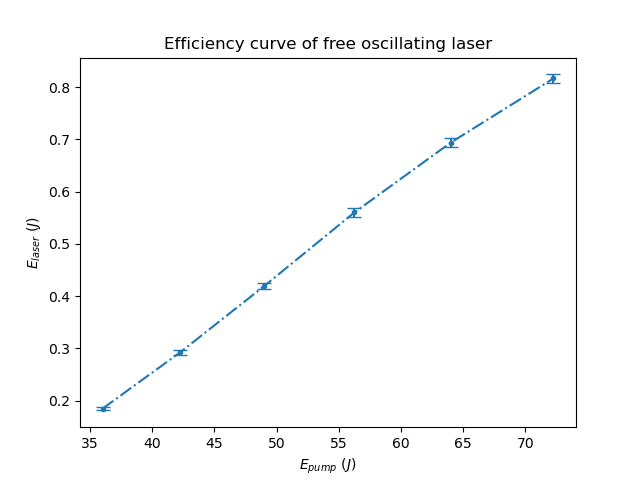
\includegraphics[width=0.9\textwidth]{./ffig1.png}
        \caption{自由震荡激光效率曲线}
    \end{minipage}
\end{figure}

\section{测量自由震荡激光脉冲波形}

在泵浦电压为$E_{pump} = 750V$时,测量自由震荡激光脉冲波形如下:

\begin{figure}[H]
    \centering
    \begin{minipage}[b]{0.9\textwidth}
        \centering
        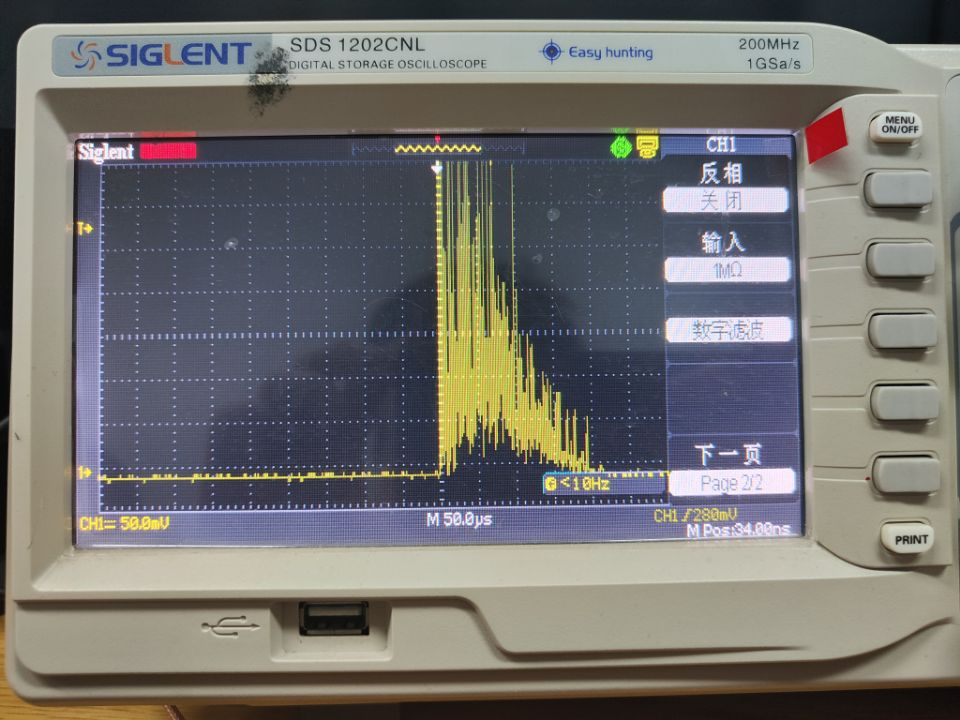
\includegraphics[width=0.9\textwidth]{./ffig2.jpg}
        \caption{$E_{pump} = 750V$时,自由震荡激光脉冲波形}
    \end{minipage}
\end{figure}

发现其半高全宽为$100\mu s$,放大后可以发现其波形为一系列尖峰脉冲:

\begin{figure}[H]
    \centering
    \begin{minipage}[b]{0.9\textwidth}
        \centering
        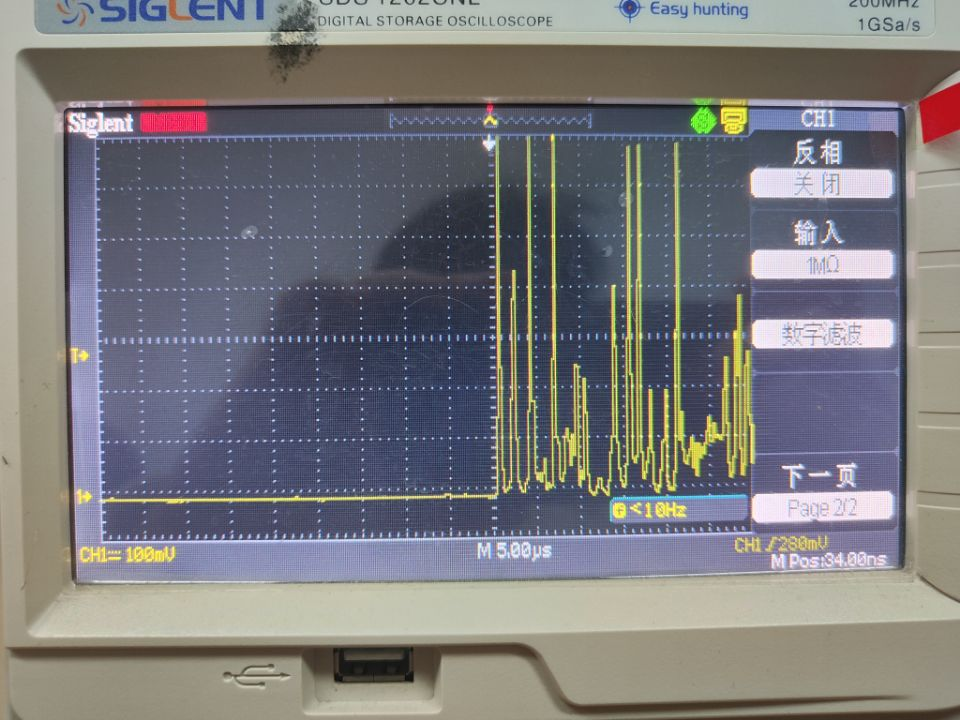
\includegraphics[width=0.9\textwidth]{./ffig3.jpg}
        \caption{$E_{pump} = 750V$时,放大后的自由震荡激光脉冲波形}
    \end{minipage}
\end{figure}

\section{染料调Q激光脉冲实验}

在泵浦电压为$E_{pump} = 700V$时,测量调Q激光脉冲波形如下:

\begin{figure}[H]
    \centering
    \begin{minipage}[b]{0.9\textwidth}
        \centering
        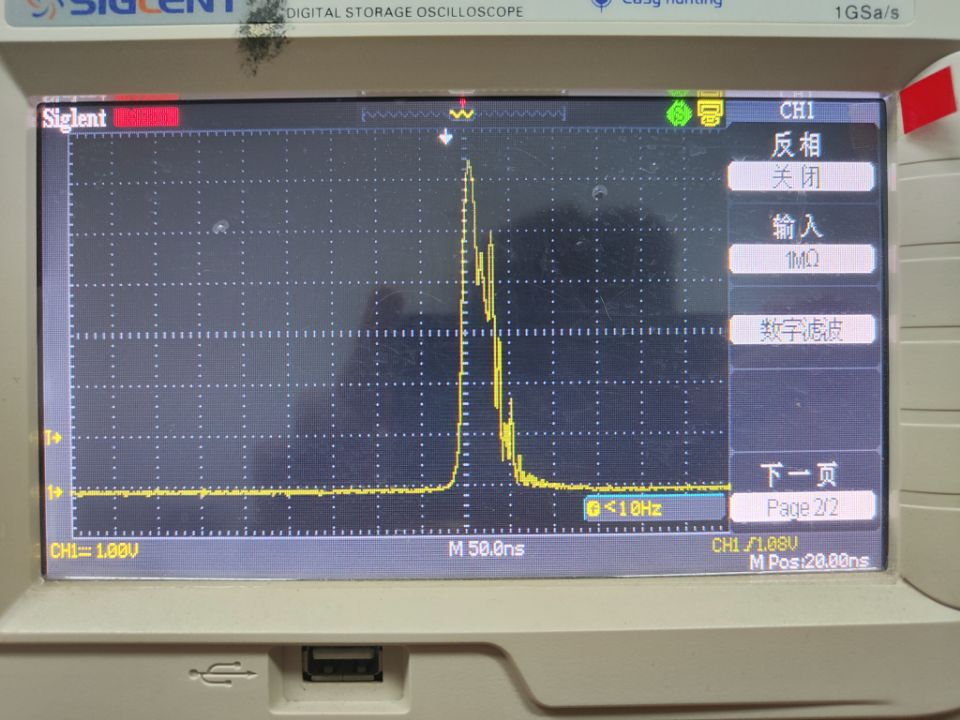
\includegraphics[width=0.7\textwidth]{./ffig4.jpg}
        \caption{$E_{pump} = 700V$时,染料调Q激光脉冲波形}
    \end{minipage}
\end{figure}

发现其半高全宽为$\Delta t_{Q} = 40 ns$

\section{DKDP电光晶体调Q激光脉冲实验}

在泵浦电压为$E_{pump} = 700V$时,测量调Q激光脉冲波形如下:

\begin{figure}[H]
    \centering
    \begin{minipage}[b]{0.9\textwidth}
        \centering
        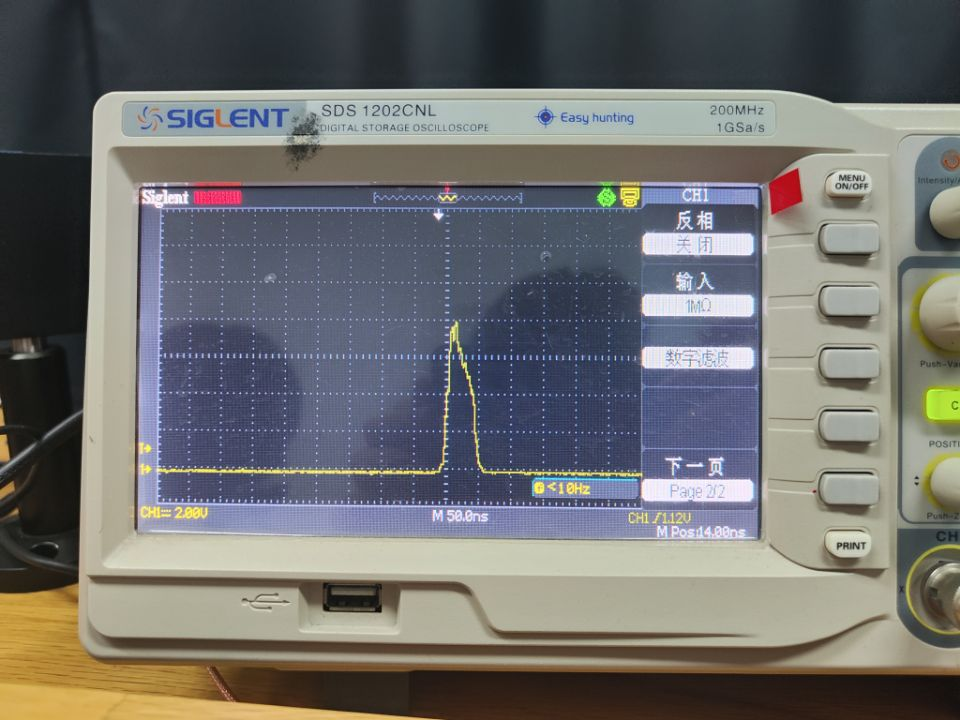
\includegraphics[width=0.7\textwidth]{./ffig5.jpg}
        \caption{$E_{pump} = 700V$时,DKDP电光调Q激光脉冲波形}
    \end{minipage}
\end{figure}

发现其半高全宽为$\Delta t_{Q} = 40 ns$

\section{双脉冲现象}

\begin{figure}[H]
    \centering
    \begin{minipage}[b]{0.9\textwidth}
        \centering
        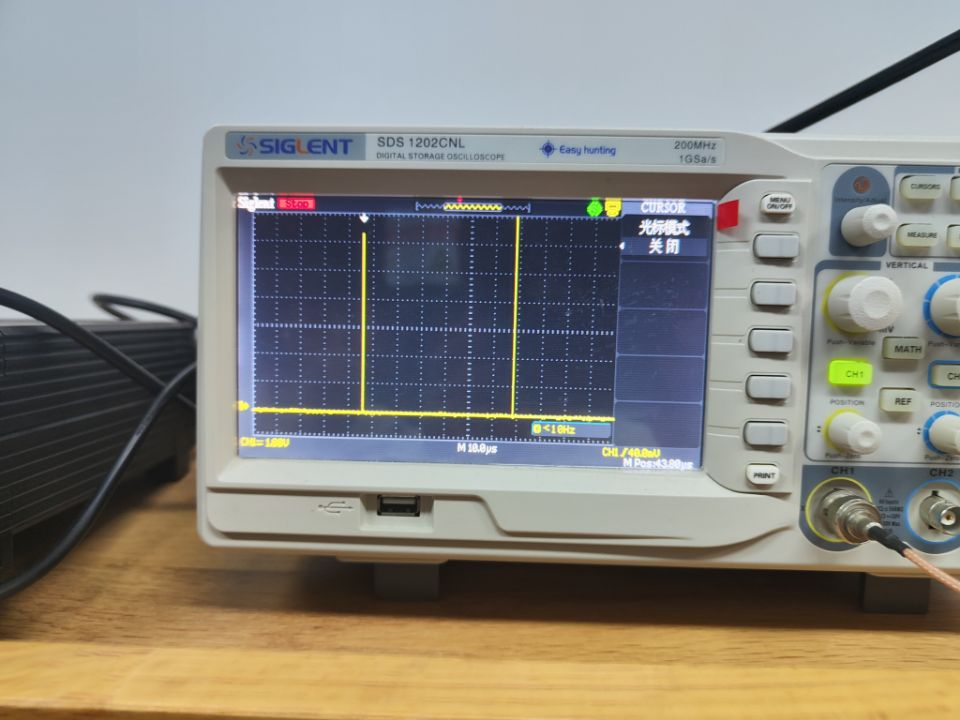
\includegraphics[width=0.9\textwidth]{./ffig6.jpg}
        \caption{$E_{pump} = 750V$时,被动调Q出现双脉冲现象}
    \end{minipage}
\end{figure}

\end{document}